\documentclass[class=book, crop=false, oneside, 12pt]{standalone}
\usepackage{standalone}
\usepackage{../../style}
\graphicspath{{./assets/images/}}

% arara: pdflatex: { synctex: yes, shell: yes }
% arara: latexmk: { clean: partial }
\begin{document}
\chapter{Analisi sintattica: bottom-up parsing}
Iniziamo la trattazione del parsing di tipo \emph{bottom-up}: come suggerisce il nome stesso, consiste nel ricostruire le derivazioni di una parola in ordine inverso, partendo dall'ultima produzione e arrivando infine allo start symbol; a livello visivo, possiamo pensare che la nostra intenzione è di partire dalle foglie di un albero di derivazione e risalirlo fino alla radice.

Possiamo subito anticipare che anche in questo approccio possiamo identificare diversi classi di grammatiche, ciascuna delle quali ci permetterà di utilizzare, di volta in volta, diverse tecniche di parsing; in ogni caso, ciascuna di queste classi condivide le seguenti caratterstiche:
\begin{itemize}
    \item per qualsiasi grammatica \(\G\) considerata, andremo sempre a espandere il suo insieme \(\P\) in \(\P'\) aggiungendo la produzione \(S \to S'\), dove \(S'\) è un non-terminale \emph{fresh};
    \item utilizzano i medesimi algoritmi \emph{shift} e \emph{reduce} (ne parleremo più avanti);
    \item hanno sempre un automa a stati finito, detto \emph{automa caratteristico}, il cui ruolo è di supervisionare il funzionamento dell'algoritmo di parsing.
\end{itemize}
Dipendentemente dalla classe di grammatica considerata, avremo automi caratteristici che rappresentano le informazioni in maniera più o meno dettagliata. Maggiore è il livello di dettaglio dell'informazione, più diventa grande e complesso l'automa caratteristico, ma anche più potente diventail nostro parsing, inteso come numero di diverse grammatiche che può analizzare. Impariamo a conoscere qual è il significato delle abbreviazioni che costituiscono quei nomi un po' criptici delle classi di grammatiche:
\begin{labeling}{LA}
    \item[L] left: leggiamo l'input da sinistra;
    \item[R] ricostruiamo una derivazione rightmost;
    \item[1] andiamo a considerare un simbolo alla volta;
    \item[LA] sta per look ahead;
    \item[S] sta per simple;  
\end{labeling}
Noi diciamo che una grammatica \(\G\) appartiene a una certa classe, ad esempio LR(1), se \(\G\) può essere costruita con la tecnica sottesa al bottom-up parsing di tipo LR(1), vale a dire quando saremo capaci di definire una tabella deterministica che ne rispetti i vincoli.

Tra quelli presentati, il meccanismo più potente è LR(1), complementare di LL(1); per questo motivo noi cercheremo sempre di costruire una tabella di parsing deterministico che rientri nei vincoli di LR(1). Se questo non sarà possibile andremo a scalare in complessità con LALR e SRL.

Andiamo ora a considerare un esempio con una delle prime grammatiche che abbiamo visto, quella che genera due occorrenza bilanciate:
\begin{equation*}
    \label{balanced}
    \G: S \to aSb \mid ab
\end{equation*}
L'automa caratterisco di tipo LR(1) per questa grammatica è il seguente:
\begin{figure}[H]
    \centering
    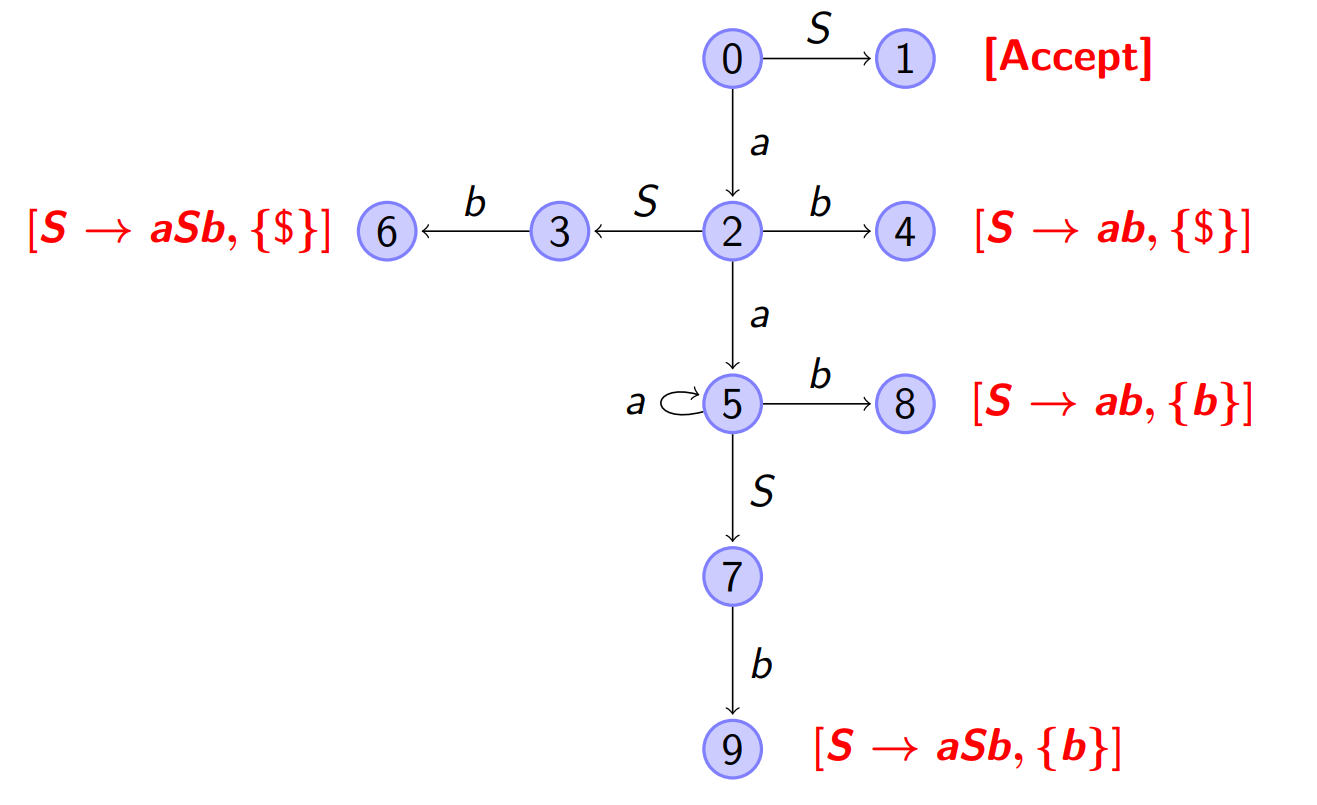
\includegraphics[width=\textwidth,keepaspectratio]{balanced-char_aut-lr1.png}
    \caption{Automa caratteristico LR(1) per Eq. \ref{balanced}}
    \label{balanced-char_aut-lr1}
\end{figure}
Lo utilizzeremo come guida per determinare, di volta in volta, quali mosse di shift e reduce applicare per verificare se una certa parola appartiene o no al linguaggio generato da \(\G\).

Consideriamo ad esempio la parola \(w = aaabbb\). Come prima cosa le applichiamo il carattere terminatore di stringa \(aaabbb\$\), e successivamente dobbiamo parlare delle strutture che utilizzeremo nella procedura, che saranno due pile:
\begin{itemize}
    \item nella prima inseriamo gli stati verso cui ci muoviamo;
    \item nella seconda conserviamo la derivazione parziale a cui siamo arrivati sinora.
\end{itemize}
Si tenga presente che in realtà potremmo farci bastare anche una sola pila, ma andrebbe a complicare sensibilmente la gestione della procedura.
\begin{itemize}
    \item Partiamo dallo stato \(0\) e inseriamolo nella pila degli stati;
    \item il primo simbolo che leggo in \(w\) è \(a\), vedo che l'automa presenta una \(a\)-transizione verso lo stato \(2\), per cui la eseguo, inserisco lo stato \(2\) nella pila, cancello il simbolo \(a\) appena "consumato" e passo al prossimo simbolo;
    \item il prossimo simbolo è ancora \(a\); di nuovo, eseguo la \(a\)-transizione verso lo stato \(5\), lo inserisco nella pila degli stati, elimino il simbolo consumato e vado avanti;
    \item abbiamo una terza occorrenza di \(a\) e abbiamo una \(a\)-transizione in forma di self loop in \(5\), che andiamo ad eseguire, reinserendo \(5\) nella pila degli stati e cancellando la nostra terza \(a\);
    \item troviamo quindi una \(b\), per cui ci spostiamo allo stato \(8\), il quale ha un'etichetta rossa, che riporta la formula \(S \to ab, \{b\}\); questo sta a indicare che, se abbiamo appena letto due simoli \(ab\), possiamo ritornare indietro di due passi, eliminando i due precedenti stati dalla pila e spostarmi direttamento dal primo \(5\) a \(7\), dal momento che i due stati sono collegati da una \(S\)-transizione:
    \begin{align*}
        \textrm{pila degli stati prima:} &\quad 02558 \\
        \textrm{pila degli stati dopo:} &\quad 0257 
    \end{align*}
    inoltre dobbiamo anche rimuovere gli ultimi due simboli \(ab\) dalla pila della derivazione e sostituirli con \(S\):
    \begin{align*}
        \textrm{pila di derivazione prima:} &\quad \#aaab \\
        \textrm{pila di derivazione dopo:} &\quad \#aaS 
    \end{align*}
    \item leggiamo un'altra \(b\) e avanziamo allo stato \(9\), e anche qui operiamo un passo di riduzione (reduce), nello specifico abbiamo che \(R: S \to aSb, \{b\}\); questo ci dice che dobbiamo tornare indietro di tre passi, eliminando i tre elementi precedenti sia nella pila degli stati e muovendoci verso \(3\), sia nella pila delle derivazioni; si osservi attentamente il cambiamento delle pile per capire cosa succede:
    \begin{align*}
        \textrm{pila degli stati prima:} &\quad 02579 & \textrm{pila di derivazione prima:} &\quad \#aaSb \\
        \textrm{pila degli stati dopo:} &\quad 023 & \textrm{pila di derivazione dopo:} &\quad \#aS
    \end{align*}
    \item proseguo quindi con la lettura e incontro una terza \(b\), mi muovo verso \(6\) e incontro una terza riduzione \(R: S \to aSb, \{\$\}\); di nuovo, torno indietro di tre stati e contestualmente sostituisco gli elementi nelle pile: 
    \begin{align*}
        \textrm{pila degli stati prima:} &\quad 0236 & \textrm{pila di derivazione prima:} &\quad \#aSb \\
        \textrm{pila degli stati dopo:} &\quad 0 & \textrm{pila di derivazione dopo:} &\quad \#S
    \end{align*}
    \item abbiamo terminato: ci troviamo nello stato \(0\) e troviamo solamente il nostro start symbol \(S\), che ci permette  muoverci verso lo stato \(1\), e l'endmaker \$; la presenza della keyword \(ACCEPT\) nello stato in cui abbiamo terminato ci indica che la parola è stata riconosciut dall'automa.
\end{itemize}
%  - Mi sposto seguendo tutte le varie x-transizioni del caso
% In pratica faccio questo:

% - Mi sposto seguendo tutte le varie x-transizioni del caso
% Se sulla pila da leggere trovo il letterale 𝑙 devo ritornare indietro a quando ho iniziato a
% leggere il body di 𝐴 → 𝐵 (ovvero 𝐵) e da quel punto leggo 𝑆 invece che 𝐵
% ○
% Quando arrivo in un certo nodo con un passo di riduzione questo mi presenterà una
% formula di questa forma 𝐴 → 𝐵,{𝑙}. -
% - Quelli descritti sopra sono passi di riduzione
% - Una volta che arrivo a leggere il terminale \$
% Gli automi caratteristici possono essere sostituiti da una tabella.
% Ora che abbiamo chiaro come fare questo parsing dobbiamo andare a capire come calcolare
% l'automa o la relativa tabella di parsing.
% Nota:
% La mossa di shift è quella che compi normalmente passando da un nodo all'altro aggiungendo
% un terminale alla pila di derivazione ed aggiungendo uno stato alla pila degli stati
% 1.
% La mossa di reduce è quella che si compie quando si arriva ad un nodo etichettato con una
% riduzione, ovvero quella mossa che ci porta ad eliminare terminali dalla pila di derivazione e
% stati dalla pila degli stati
% 2.
% Quello che abbiamo visto è l'algoritmo di shift/reduce
% Per la cronaca: l'automa visto era del tipo LR(1)
% #Automa caratteristico: come è fatto?
% Gli stati sono insiemi di item
% - LR(0)-items 𝐴 → 𝛼 ⋅ 𝛽
% - LR(1)-items 𝐴 → 𝛼 ⋅ 𝛽, 𝐿 dove 𝐿 ⊂= 𝑇 ∪ {\$}
% Gli item sono:
% Come detto in precedenza gli LR(1) items contengono più informazioni e sono più ricchi degli LR(0) e
% ci permettono di riconoscere più grammatiche
% Comunque il livello 0 dell'item è caratterizzato da una produzione con un punto EHHH?
% Consideriamo ora l'item LR(0) 𝑆
% ᇱ → ⋅ 𝑆
% Il significato intuitivo è:
% Se sono all'origine del parsing è come dire che mi trovo in una posizione da cui voglio vedere
% qualcosa che sia derivabile dalla 𝑆. Quindi è logico pensare come l'item 𝑆
% ᇱ →⋅ 𝑆 deve stare nello stato iniziale dell'automa, diciamo
% 𝑃଴ . Ma questo non è l'unico item che deve stare in quello stato:
% Se io devo vedere qualcosa che deriva dalla S nella mia grammatica precedente mi aspetto di vedere
% qualcosa che deriva da 𝑎𝑆𝑏 o che deriva da 𝑎𝑏. Quindi gli LR(0) items di 𝑆 saranno
% 𝑆 → ⋅ 𝑎𝑆𝑏
% 𝑆 → ⋅ 𝑎𝑏

% 𝑆 → ⋅ 𝑎𝑏
% Vediamo ora il concetto di chiusura di set di LR(0)-items
% Sia 𝑃 un set di LR(0)-items
% 𝑐𝑙𝑜𝑠𝑢𝑟𝑒଴(𝑃) è il più piccolo set che soddisfa la seguente equazione
% 𝑐𝑙𝑜𝑠𝑢𝑟𝑒଴
% (𝑃) = 𝑃 ∪ {𝐵 → ⋅ 𝛾 𝑡𝑎𝑙𝑒 𝑐ℎ𝑒 𝐴 → 𝛼 ⋅ 𝐵𝛽 ∈ 𝑐𝑙𝑜𝑠𝑢𝑟𝑒଴
% (𝑃) 𝑎𝑛𝑑 𝐵 → 𝛾 ∈ 𝑃
% ᇱ}
% Tale formula si traduce con il seguente algoritmo:
% Testiamo l'algoritmo:
% 𝑆
% ᇱ → . 𝑆
% Ci aspettiamo quindi di vedere qualcosa che deriva dalla S, ovvero:
% 𝑆 → . 𝑎𝑆𝑏
% 𝑆 → . 𝑎𝑏
% L'insieme 𝑐𝑙𝑜𝑠𝑢𝑟𝑒଴(𝑆′) in questo caso è proprio
% 𝑆
% ᇱ → . 𝑆
% 𝑆 → . 𝑎𝑆𝑏
% 𝑆 → . 𝑎𝑏
% Perché tutte le espansioni possibili sono inserite già in 𝑃
% Se avessimo invece
% 𝑆 → 𝑎. 𝑆𝑏
% 𝑆 → . 𝑎𝑆𝑏
% 𝑆 → . 𝑎𝑏
% La prima riga ci dice che abbiamo già visto una a ed ora ci aspettiamo di vedere qualcosa che deriva
% da Sb e così via.
% La chiusura consiste sostanzialmente in tutti gli item che hanno un punto davanti ad un non
% terminale. Poi ricorsivamente si vanno ad aggiungere tutte le chiusure dei terminali con un punto
% davanti.

\end{document}